%TCIDATA{LaTeXparent=0,0,cap_RevisaoBibliografica.tex}

\section{Simula\c{c}\~{a}o Num\'{e}rica de Reservat\'{o}rios}
\subsection{Vis\~{a}o Geral}
A simula\c{c}\~{a}o num\'{e}rica de um reservat\'{o}rio \'{e}, segundo Peaceman, \'{e} o processo de infer\^{e}ncia do comportamento do reservat\'{o}rio real dada a performance obtida de um modelo do mesmo, matem\'{a}tico ou f\'{i}sico (em escala laboratorial). Um modelo matem\'{a}tico de reservat\'{o}rio pode ser enxergado como um conjunto de equa\c{c}\~{o}es diferenciais parciais, juntamente com as condi\c{c}\~{o}es de contorno adequadas, que podem ser utilizadas para descrever satisfatoriamente os processos f\'{i}sicos importantes que ocorrem no sistema real. Os processos que ocorrem em um reservat\'{o}rio s\~{a}o basicamente transporte de fluidos e transfer\^{e}ncia de massa; at\'{e} tr\^{e}s fases imisc\'{i}veis (\'{o}leo, g\'{a}s e \'{a}gua) fluem simultaneamente, enquanto que o transporte de massa se d\'{a} entre as fases (notadamente entre o \'{o}leo e o g\'{a}s). A gravidade, a capilaridade e as for\c{c}as viscosas s\~{a}o tamb\'{e}m importantes no processo de vaz\~{a}o dos fluidos \cite{simres}.

Al\'{e}m da defini\c{c}\~{a}o proposta por Peaceman, Heimsund descreve a simula\c{c}\~{a}o de reservat\'{o}rios como uma ferramenta de investiga\c{c}\~{a}o da vaz\~{a}o de fluidos em subsuperf\'{i}cie. O autor destaca que as simula\c{c}\~{o}es de reservat\'{o}rio abrangem \'{a}reas relacionadas a ramos importantes da ci\^{e}ncia, como matem\'{a}tica, f\'{i}sica, qu\'{i}mica, geologia e biologia; al\'{e}m disso, afirma que, na ind\'{u}stria petrol\'{i}fera, os principais usos dos simuladores de reservat\'{o}rios envolvem a obten\c{c}\~{a}o de esquemas \'{o}timos de explota\c{c}\~{a}o e predi\c{c}\~{a}o da produ\c{c}\~{a}o\cite{heimsund2005}. J\'{a} Dake afirma que um simulador num\'{e}rico de reservat\'{o}rio \'{e} um programa de computador em que o sistema estudado \'{e} dividido em v\'{a}rias c\'{e}lulas discretas, cujas propriedades podem ser diferentes entre si \cite{dake}.

Segundo Rosa, a primeira etapa de uma simula\c{c}\~{a}o num\'{e}rica \'{e} formular o problema f\'{i}sico a ser representado matematicamente; em seguida s\~{a}o feitas suposi\c{c}\~{o}es e simplifica\c{c}\~{o}es compat\'{i}veis com o grau de sofistica\c{c}\~{a}o esperado do modelo, levando-se \`{a} formula\c{c}\~{a}o das equa\c{c}\~{o}es matem\'{a}ticas que descrevem o problema desejado, considerando-se as hip\'{o}teses adotadas. O passo seguinte \'{e} a resolu\c{c}\~{a}o das equa\c{c}\~{o}es e an\'{a}lise da solu\c{c}\~{a}o obtida; posteriormente, a validade do simulador \'{e} verificada atrav\'{e}s da calibra\c{c}\~{a}o com uma solu\c{c}\~{a}o existente --- por exemplo, comparam-se os resultados obtidos do simulador num\'{e}rico com solu\c{c}\~{o}es anal\'{i}ticas, resultados reais ou com resultados obtidos de modelos f\'{i}sicos de laborat\'{o}rio (dados experimentais). Caso o simulador seja considerado v\'{a}lido, o mesmo estar\'{a} pronto para ser utilizado na simula\c{c}\~{a}o do fen\^{o}meno desejado; caso contr\'{a}rio, volta-se para um novo ciclo em que s\~{a}o revistas as hip\'{o}teses adotadas ou at\'{e} a conceitua\c{c}\~{a}o do modelo f\'{i}sico \cite[p. 520]{engres}. A Figura \ref{fig:rev_simuesq} esquematiza um desenvolvimento b\'{a}sico de um simulador num\'{e}rico qualquer, enquanto que a Figura \ref{fig:rev_simuex} mostra uma compara\c{c}\~{a}o de resultados entre diferentes simuladores existentes, exemplificando o uso da calibra\c{c}\~{a}o com solu\c{c}\~{o}es j\'{a} obtidas para se validar um simulador de reservat\'{o}rio. 

\begin{figure}[H]
\centering
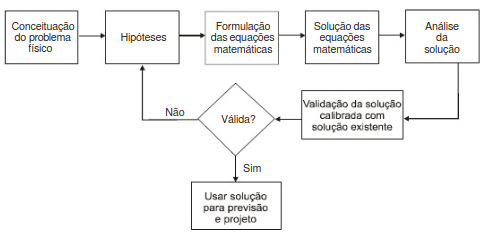
\includegraphics[width=.75\textwidth]{figs/revisao/revisao_simuesq.png}
\caption{Esquema b\'{a}sico de desenvolvimento de um simulador num\'{e}rico de reservat\'{o}rio \cite[p. 519]{engres}.}\label{fig:rev_simuesq}
\end{figure}

\begin{figure}[H]
\centering
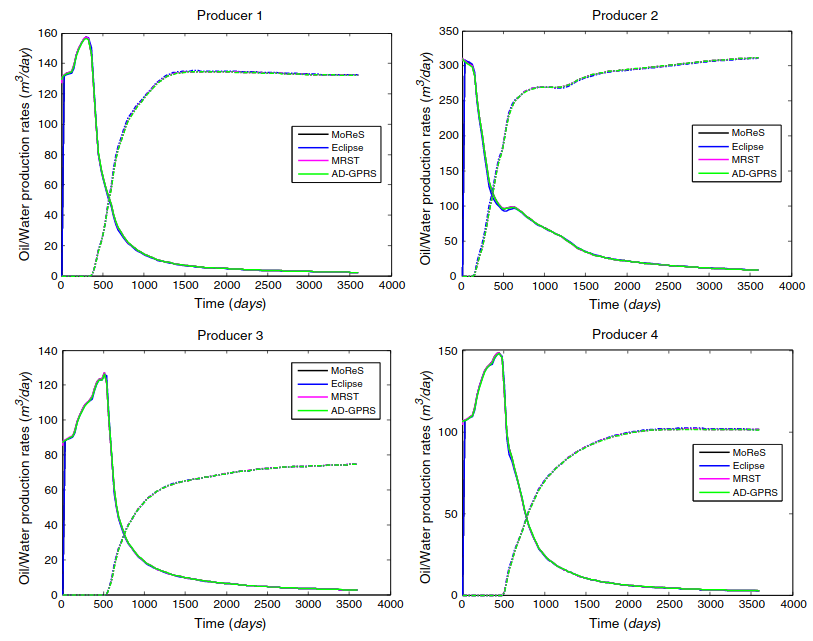
\includegraphics[width=.75\textwidth]{figs/revisao/revisao_simuex.png}
\caption{Exemplo de compara\c{c}\~{a}o de dados entre simuladores de vaz\~{a}o de \'{a}gua e de \'{o}leo de um modelo \cite{eggM}.}\label{fig:rev_simuex}
\end{figure}

\subsection{Hist\'{o}ria da Simula\c{c}\~{a}o de Reservat\'{o}rios}
Para se tra\c{c}ar a evolu\c{c}\~{a}o da simula\c{c}\~{a}o de reservat\'{o}rios ao longo da hist\'{o}ria, consideram-se aqui, inicialmente, fatos apresentados por Coats e por Breitenbach; de acordo com Coats, a simula\c{c}\~{a}o de reservat\'{o}rios \'{e} praticada desde o surgimento da engenharia de petr\'{o}leo, durante a d\'{e}cada de 1930. J\'{a} na d\'{e}cada de 1940, segundo Breitenbach, a simula\c{c}\~{a}o de reservat\'{o}rios passa a ser reconhecida, com as companhias desenvolvendo m\'{e}todos anal\'{i}ticos e num\'{e}ricos para a melhoria das solu\c{c}\~{o}es anal\'{i}ticas resistentes, balan\c{c}o de materiais e c\'{a}lculo de posicionamento 1-D de Buckley-Leverett; na d\'{e}cada seguinte (1950), as pesquisas por solu\c{c}\~{o}es num\'{e}ricas das equa\c{c}\~{o}es de vaz\~{a}o come\c{c}am a surtir efeito, com o surgimento de programas computacionais rudimentares, por\'{e}m eficientes, de simula\c{c}\~{o}es de reservat\'{o}rios. Considera-se um grande avan\c{c}o o surgimento dessas solu\c{c}\~{o}es, em que foi poss\'{i}vel resolver equa\c{c}\~{o}es de diferen\c{c}as finitas em modelos 2D e 3D, al\'{e}m de simula\c{c}\~{o}es em meios de porosidade heterog\^{e}nea; enfim, problemas mais complexos de engenharia de reservat\'{o}rio podiam ser resolvidos\footnote{Ver \cite{coats1982} e \cite{breitenbach1991}}.

A d\'{e}cada de 1960 representou, segundo Coats, um marco importante, em que a palavra ``simula\c{c}\~{a}o'' se torna comum, \`{a} medida em que os programas destinados \`{a} resolu\c{c}\~{a}o de problemas de reservat\'{o}rios se tornavam mais sofisticados; durante essa d\'{e}cada, os esfor\c{c}os na busca de simuladores melhores de reservat\'{o}rios se concentraram em modelos bif\'{a}sicos de g\'{a}s/\'{a}gua e \textit{black-oil} trif\'{a}sicos; os m\'{e}todos de recupera\c{c}\~{a}o de \'{o}leo simulados se restringiam essencialmente \`{a} deple\c{c}\~{a}o ou manuten\c{c}\~{a}o da press\~{a}o. Era poss\'{i}vel, na \'{e}poca, o desenvolvimento de um \'{u}nico modelo de simula\c{c}\~{a}o que conseguia tratar de quase todos os problemas de reservat\'{o}rios encontrados, o que sempre atraiu o interesse das companhias operadoras do ramo por conta da redu\c{c}\~{a}o de custos com treinamento e uso e, potencialmente, de custos de manuten\c{c}\~{a}o e desenvolvimento do modelo \cite{coats1982}.

Para se entender o rumo das simula\c{c}\~{o}es de reservat\'{o}rio na d\'{e}cada de 1970, \'{e} importante considerar o momento hist\'{o}rico; nessa \'{e}poca, ocorria o embargo da OPEP (Organiza\c{c}\~{a}o dos Pa\'{i}ses Exportadores de Petr\'{o}leo), acarretando um aumento brusco do pre\c{c}o do petr\'{o}leo. Esse embargo, segundo Brosche, ocorreu como uma repres\'{a}lia dos pa\'{i}ses \'{a}rabes aos Estados Unidos e \`{a} Uni\~{a}o Europeia, devido ao apoio dos mesmos ao Estado de Israel durante as guerras que afetaram o Oriente M\'{e}dio, uma regi\~{a}o rica em petr\'{o}leo; o embargo se deu logo ap\'{o}s a guerra do Yom Kippur, em 1973 \cite{brosche1974}. Durante esse per\'{i}odo, ocorre a prolifera\c{c}\~{a}o dos m\'{e}todos de EOR, como inje\c{c}\~{o}es misc\'{i}veis, qu\'{i}micas, de $CO_2$ e vapor, al\'{e}m da combust\~{a}o \textit{in-situ}; os simuladores, portanto, passaram a considerar esses m\'{e}todos de recupera\c{c}\~{a}o, al\'{e}m de adicionar aos modelos efeitos t\'{e}rmicos e comportamentos complexos de equil\'{i}brio de fase. A estrat\'{e}gia de se manter um modelo \'{u}nico de reservat\'{o}rio, devido ao advento dos m\'{e}todos de EOR, foi modificada com a ideia de se obter v\'{a}rios modelos reproduzindo o comportamento do sistema estudado em resposta aos m\'{e}todos de recupera\c{c}\~{a}o de \'{o}leo aplicados. Pode-se afirmar, portanto, que a d\'{e}cada de 1970 representou um avan\c{c}o significativo no esfor\c{c}o de se obter simula\c{c}\~{o}es mais complexas, com custo computacional reduzido e melhor efici\^{e}ncia das solu\c{c}\~{o}es num\'{e}ricas \cite{coats1982}.

Durante a d\'{e}cada de 1980, a expans\~{a}o da gama de aplica\c{c}\~{o}es envolvendo simula\c{c}\~{a}o de reservat\'{o}rios continuou, segundo Breitenbach; os avan\c{c}os da \'{e}poca incluem o uso de geoestat\'{i}stica para descrever, por exemplo, heterogeneidades, a tecnologia para a modelagem de reservat\'{o}rios naturalmente fraturados, incluindo efeitos composicionais, com extens\~{o}es na simula\c{c}\~{a}o de fraturamento hidr\'{a}ulico, po\c{c}os horizontais e aplica\c{c}\~{o}es em processos complexos como monitoramento de reservat\'{o}rio \cite{breitenbach1991}\footnote{Breitenbach ainda afirma que, no final da d\'{e}cada de 1980, as simula\c{c}\~{o}es de reservat\'{o}rios passam tamb\'{e}m a ser executadas em computadores pessoais.}. Nessa \'{e}poca, afirmam Lucia \textit{et al.}, o n\'{i}vel de maturidade da pesquisa envolvendo simula\c{c}\~{a}o de reservat\'{o}rios chegou ao ponto de se tornar um t\'{o}pico presente em trabalhos da SPE (/\textit{Society of Petroleum Engineers}). Os autores ainda afirmam que, no come\c{c}o do s\'{e}culo XXI, a simula\c{c}\~{a}o de reservat\'{o}rios chegou ao ponto de se considerar ferramentas de modelagem baseadas em coneitos mais avan\c{c}ados, entre os quais incluem-se modelos de porosidade dual, considera\c{c}\~{o}es de balan\c{c}o de energia, comportamento rigoroso de fase, entre outros  \cite{luciaetal}.

\'{E} poss\'{i}vel afirmar que a evolu\c{c}\~{a}o da simula\c{c}\~{a}o est\'{a} diretamente atrelada \`{a} evolu\c{c}\~{a}o da computa\c{c}\~{a}o; analisando-se as considera\c{c}\~{o}es feitas por Coats, Breitenbach e Lucia \textit{et al.}, percebe-se que os avan\c{c}os obtidos na \'{a}rea se tornaram poss\'{i}veis \`{a} medida em que os computadores se tornaram menores, por\'{e}m mais r\'{a}pidos. Atualmente, a simula\c{c}\~{a}o de reservat\'{o}rios chegou a um n\'{i}vel em que os mais variados modelos de reservat\'{o}rio, n\~{a}o necessariamente os mais simples, podem ser simulados com um computador pessoal, como \'{e} o caso nesta pesquisa.

\subsection{Leis F\'{i}sicas Consideradas}

No caso de um simulador de reservat\'{o}rios, as seguintes leis f\'{i}sicas b\'{a}sicas normalmente s\~{a}o consideradas, dependendo do tipo de simulador\footnote{Ver \cite[p. 520]{engres}}:

\begin{itemize}
\item Lei da conserva\c{c}\~{a}o de massa;
\item Lei da conserva\c{c}\~{a}o de energia;
\item Lei da conserva\c{c}\~{a}o de \textit{``momentum''} (Segunda Lei de Newton):
\begin{equation}
\sum F = \frac{\partial M}{\partial t},
\end{equation}
onde $F$ representa uma for\c{c}a e $M = mv$ o \textit{``momentum''}, com $m$ sendo a massa e $v$ a velocidade.
\end{itemize}

De um modo geral, na modelagem de fen\^{o}menos f\'{i}sicos, considera-se importante o estudo das equa\c{c}\~{o}es de conserva\c{c}\~{a}o; segundo Heimsund, o princ\'{i}pio da conserva\c{c}\~{a}o pode ser generalizado tomando-se uma vari\'{a}vel quantitativa $u$ contida em um volume de controle fixo $\Omega$. A vari\'{a}vel $u$ pode ser modificada dentro de $\Omega$ por um dado fluxo $\vec{F}$ sobre a superf\'{i}cie de contorno $\Gamma$ de $\Omega$. A conserva\c{c}\~{a}o de $u$ pode ser escrita, na sua forma integral, como
\begin{equation}
	\int_{\Omega} \frac{\partial u}{\partial t}dV ~+~\oint_{\Gamma}\vec{F}\cdot\vec{n}dS = \int_{\Omega} Q dV,
\end{equation}
em que $Q$ pode ser encarado como uma fonte ($Q > 0$) ou dreno ($Q < 0$). A integral de superf\'{i}cie pode ser convertida, utilizando-se o teorema de Gauss; portanto, a equa\c{c}\~{a}o da conserva\c{c}\~{a}o de $u$ pode ser reescrita como
\begin{equation}
\int_{\Omega} \frac{\partial u}{\partial t}dV + \int_{\Omega} \nabla\cdot\vec{F} dV = \int_{\Omega}Q dV
\end{equation}
\begin{equation}\label{consU}
\int_{\Omega} \left(\frac{\partial u}{\partial t} + \nabla\cdot\vec{F} - Q \right)dV = 0.
\end{equation}
Como a Equa\c{c}\~{a}o \eqref{consU} deve valer para qualquer tamanho de $\Omega$, a integral pode ser omitida da equa\c{c}\~{a}o:
\begin{equation}\label{consU2}
\frac{\partial u}{\partial t} + \nabla\cdot\vec{F} = Q.
\end{equation}
No caso da modelagem de fluxo em reservat\'{o}rio, a vari\'{a}vel $u$ pode ser, por exemplo, a massa de uma dada fase (\'{a}gua, \'{o}leo ou g\'{a}s), a massa molecular das subst\^{a}ncias ou a energia t\'{e}rmica \cite{heimsund2005}.

Al\'{e}m das leis b\'{a}sicas da f\'{i}sica, faz-se necess\'{a}rio o uso de v\'{a}rias leis, dependendo do simulador, que governam o comportamento dos fluidos envolvidos e a propriedade do reservat\'{o}rio estudado, apresentadas nas subse\c{c}\~{o}es a seguir\footnote{Os teoremas apresentados se encontram em \cite[pp. 520-522]{engres}}. Combinado-se as equa\c{c}\~{o}es correspondentes \`{a}s leis b\'{a}sicas, obt\'{e}m-se uma equa\c{c}\~{a}o diferencial parcial que rege o comportamento das vari\'{a}veis dependentes em fun\c{c}\~{a}o das vari\'{a}veis independentes e dos par\^{a}metros do sistema. Como normalmente a equa\c{c}\~{a}o obtida \'{e} n\~{a}o-linear, ela \'{e}, consequentemente, \'{e} resolvida por m\'{e}todos n\'{u}mericos; da\'{i} a nomenclatura \textit{simula\c{c}\~{a}o num\'{e}rica de reservat\'{o}rios}. 

\subsubsection{Fen\^{o}menos de Transporte}

\begin{theorem}[Lei de Darcy]
Na Lei de Darcy, ou lei do fluxo ``laminar'' ou Darcyano, a velocidade do fluxo viscoso de um fluido em meio poroso \'{e} dada por
\begin{equation}
	v_s = -\frac{k_s}{\mu} \frac{\partial\Phi}{\partial s},
\end{equation}
onde $k$ \'{e} a permeabilidade efetiva do meio ao fluido considerado, $\mu$ \'{e} a viscosidade do fluido, $\Phi$ \'{e} o potencial de fluxo e $s$ \'{e} a trajet\'{o}ria de fluxo.
\end{theorem}

\begin{theorem}[Lei de Forchheimer]
Tamb\'{e}m conhecida como lei do fluxo ``turbulento'' ou n\~{a}o-Darcyano, \'{e} utilizada para fluxos turbulentos, notadamente de g\'{a}s; o gradiente de press\~{a}o \'{e} dado por
\begin{equation}
	-\frac{dp}{ds} = \frac{\mu}{k_s}v_s - \beta\rho v_s^2,
\end{equation}
onde $\rho$ \'{e} a massa espec\'{i}fica do fluido e $\beta$ \'{e} o coeficiente de resist\^{e}ncia inercial ou de fluxo n\~{a}o-Darcyano. 
\end{theorem}

\begin{theorem}[Lei de Fourier]
Durante um fen\^{o}meno de transporte de calor por condu\c{c}\~{a}o, o fluxo de calor \'{e} dado por
\begin{equation}
	q_s = -k'\frac{\partial T}{\partial s},
\end{equation}
em que $k'$ \'{e} a condutividade t\'{e}rmica do meio e $T$ \'{e} a temperatura.
\end{theorem}

\begin{theorem}[Convec\c{c}\~{a}o]
O fluxo de calor no caso de tranporte por convec\c{c}\~{a}o \'{e} dado por
\begin{equation}
	q_s = c_p v_s (T - T_0),
\end{equation}
onde $c_p$ \'{e} a capacidade calor\'{i}fica do fluido \`{a} press\~{a}o constante, $v$ a velocidade do fluido e $T_0$ uma temperatura de refer\^{e}ncia.
\end{theorem}

\subsubsection{Equa\c{c}\~{o}es de Estado}
As principais equa\c{c}\~{o}es de estado envolvidas na simula\c{c}\~{a}o do comportamento de um reservat\'{o}rio de petr\'{o}leo s\~{a}o as que lidam com fluidos (l\'{i}quidos ou gasosos) e rochas porosas. No caso de fluidos l\'{i}quidos, tem-se a seguinte defini\c{c}\~{a}o:

\begin{definition}
A compressibilidade isot\'{e}rmica de um fluido \'{e} dada por
\begin{equation}
	c = -\frac{1}{V}\frac{\partial V}{\partial p} = \frac{1}{\rho}\frac{\partial \rho}{\partial p},
\end{equation}
em que $V$ \'{e} o volume, $p$ \'{e} a press\~{a}o e $\rho$ \'{e} a massa espec\'{i}fica do fluido. H\'{a} algumas rela\c{c}\~{o}es especiais para situa\c{c}\~{o}es particulares:
\begin{itemize}
\item L\'{i}quidos de compressibilidade constante: $\rho = \rho_0 e^{c(p-p_0)}$.
\item L\'{i}quidos de compressibilidade constante e pequena: $\rho = \rho_0 \left[1+c\left(p-p_0\right)\right]$.
\end{itemize}
\end{definition}

Quando se trata de estudar o estado de um g\'{a}s, se aplica a lei dos gases:
\begin{equation}\label{eq:gaslaw}
	\rho = \frac{pM}{ZRT}.
\end{equation}

A Equa\c{c}\~{a}o \eqref{eq:gaslaw} pode ser aplicada tanto no caso de um g\'{a}s real quanto de um g\'{a}s ideal; nela, $\rho$ \'{e} a massa espec\'{i}fica do g\'{a}s, $p$ \'{e} a press\~{a}o, $M$ \'{e} a massa molecular, $R$ \'{e} a constante universal dos gases, $T$ \'{e} a temperatura e $Z$ \'{e} o fator de compressibilidade do g\'{a}s; no caso de um g\'{a}s ideal, tem-se $Z = 1$.

Por fim, para se representar o comportamento da rocha, utiliza-se a equa\c{c}\~{a}o da chamada compressibilidade efetiva:
\begin{equation}
	c_f = \frac{1}{\phi} \frac{\partial\phi}{\partial p},
\end{equation}
onde $c_f$ \'{e} a compressibilidade efetiva efetiva da forma\c{c}\~{a}o e $\phi$, sua porosidade.

Al\'{e}m das leis at\'{e} aqui citadas, cabe ressaltar que outras podem ser utilizadas em caso de simula\c{c}\~{o}es de fen\^{o}menos espec\'{i}ficos, como inje\c{c}\~{a}o de vapor, inje\c{c}\~{a}o de pol\'{i}meros, al\'{e}m de outros m\'{e}todos empregados na produ\c{c}\~{a}o de petr\'{o}leo.

\subsection{Tipos de Simuladores}
Segundo Rosa, os simuladores de reservat\'{o}rios podem ser classificados em fun\c{c}\~{a}o de tr\^{e}s crit\'{e}rios b\'{a}sicos: o tratamento matem\'{a}tico utilizado, o n\'{u}mero de dimens\~{o}es consideradas e o n\'{u}mero de fases admitidas. Em rela\c{c}\~{a}o \`{a} matem\'{a}tica do simulador, os simuladores podem ser classificados em: 

\begin{itemize}
	\item \textbf{Modelo Beta ou volum\'{e}trico:} \'{e} tamb\'{e}m conhecido como \textit{black oil}; nesse modelo, s\~{a}o consideradas as fun\c{c}\~{o}es de press\~{a}o e da temperatura do reservat\'{o}rio. Al\'{e}m disso, cada fase presente no reservat\'{o}rio (\'{a}gua, \'{o}leo e/ou g\'{a}s) \'{e} admitida como constitu\'{i}da por apenas um componente, mesmo que, na pr\'{a}tica, o \'{o}leo seja composto por v\'{a}rios hidrocarbonetos, al\'{e}m de impurezas. Coats destaca que o modelo \textit{black-oil} \'{e} frequentemente utilizado na estimativa do efeito de v\'{a}rios par\^{a}metros envolvidos na recupera\c{c}\~{a}o de \'{o}leo, a saber: o espa\c{c}amento e posicionamento dos po\c{c}os, intervalos de completa\c{c}\~{a}o dos po\c{c}os, o fen\^{o}meno do cone de g\'{a}s/\'{a}gua em fun\c{c}\~{a}o da vaz\~{a}o, a vaz\~{a}o de produ\c{c}\~{a}o, refor\c{c}o do mecanismo de influxo de \'{a}gua por meio da inje\c{c}\~{a}o do mesmo fluido e a prefer\^{e}ncia por injetar \'{a}gua em regi\~{o}es perif\'{e}ricas do reservat\'{o}rio ao inv\'{e}s de padr\~{o}s de inje\c{c}\~{a}o, \textit{infill drilling} e inje\c{c}\~{a}o de \'{a}gua \textit{versus} inje\c{c}\~{a}o de g\'{a}s \textit{versus} inje\c{c}\~{a}o de \'{a}gua e g\'{a}s \cite{coats1982}. 
	\item \textbf{Modelo composicional:} Al\'{e}m de considerar a press\~{a}o e a temperatura do reservat\'{o}rio, tamb\'{e}m se admite as composi\c{c}\~{o}es das diversas fases que estejam presentes no meio poroso. Ao contr\'{a}rio do \textit{black oil}, por exemplo, o \'{o}leo passa a ser tratado pelos seus v\'{a}rios hidrocarbonetos de que \'{e} composto, tais como $C_1$, $C_2$, $C_3$, etc. Por\'{e}m, como o n\'{u}mero de componentes no \'{o}leo \'{e} grande, alguns hidrocarbonetos s\~{a}o agrupados nos chamados \textit{pseudocomponentes}; a utiliza\c{c}\~{a}o dessa abordagem reduz o tempo computacional necess\'{a}rio ao modelo, uma vez que um tratamento mais rigoroso poderia tornar impratic\'{a}vel a simula\c{c}\~{a}o composicional. Young destaca que problemas que requerem o uso de modelos composicionais s\~{a}o os que envolvem recupera\c{c}\~{a}o prim\'{a}ria ou secund\'{a}ria por inje\c{c}\~{a}o em reservat\'{o}rios de \'{o}leo vol\'{a}til ou g\'{a}s condensado, al\'{e}m de situa\c{c}\~{o}es de uso de t\'{e}cnicas de EOR envolvendo inje\c{c}\~{a}o de $CO_2$ ou de g\'{a}s enriquecido. O autor ainda sugere que \`{a} medida em que as perfura\c{c}\~{o}es tornam-se profundas, o n\'{u}mero de reservat\'{o}rios cujas condi\c{c}\~{o}es s\~{a}o melhor explicadas por modelos composicionais aumentou, al\'{e}m da necessidade de se recorrer a t\'{e}cnicas de inje\c{c}\~{a}o de g\'{a}s \cite{young1983}. 
	\item \textbf{Modelo t\'{e}rmico:} \'{e} utilizado quando \'{e} necess\'{a}rio considerar os efeitos de varia\c{c}\~{o}es t\'{e}rmica no interior do reservat\'{o}rio --- por exemplo, quando se estuda a aplica\c{c}\~{a}o de m\'{e}todos t\'{e}rmicos de recupera\c{c}\~{a}o secund\'{a}ria, como inje\c{c}\~{a}o de vapor, inje\c{c}\~{a}o de \'{a}gua quente ou combust\~{a}o \textit{in situ}. Como os modelos t\'{e}rmicos tratam situa\c{c}\~{o}es complexas, eles s\~{a}o necessariamente composicionais. Um exemplo de uso dos modelos t\'{e}rmicos \'{e} apresentado por Lucia \textit{et al.}, em que os mesmos s\~{a}o utilizados em um estudo comparativo de t\'{e}cnicas de EOR envolvendo inje\c{c}\~{a}o de vapor e uma tecnologia denominada \textit{Solvent Thermal Resource Innovation Process} (STRIP), em que a gera\c{c}\~{a}o de vapor \'{e} realizada \textit{in-situ} com a combust\~{a}o de metano \cite{luciaetal}\footnote{Ver tamb\'{e}m \cite{ZAYDULLIN201451}}.
\end{itemize}

Quanto ao n\'{u}mero de dimens\~{o}es, os simuladores s\~{a}o classificados de acordo com o n\'{u}mero de dimens\~{o}es nas quais se admite fluxo. Neste sentido, eles podem ser classificados em \textit{unidimensionais}, \textit{bidimensionais} e \textit{tridimensionais}; a Figura \ref{fig:revisao_DIM} mostra cada um desses tipos de simuladores. Por fim, os simuladores num\'{e}ricos podem ser classificados de acordo com o n\'{u}mero de fases: \textit{monof\'{a}sicos}, caso haja apenas uma fase (no caso de \'{a}gua, se trata de um aqu\'{i}fero); \textit{bif\'{a}sicos}, quando h\'{a} duas fases presentes (\'{a}gua e \'{o}leo, no caso de reservat\'{o}rios de \'{o}leo, ou \'{a}gua e g\'{a}s, nos reservat\'{o}rios de g\'{a}s); e \textit{trif\'{a}sicos}, no caso da exist\^{e}ncia de tr\^{e}s fases (\'{a}gua, \'{o}leo e gas)\footnote{A classifica\c{c}\~{a}o dos modelos de simula\c{c}\~{a}o podem ser encontradas em \cite[pp. 517--519]{engres}}.

\begin{figure}[!ht]
	\centering
	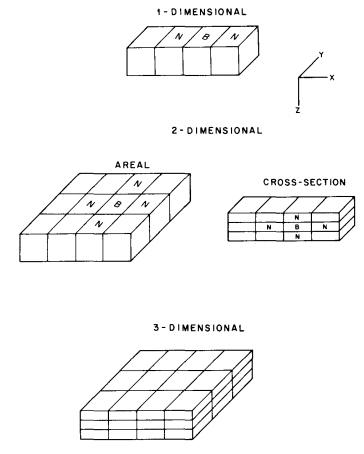
\includegraphics[width=.6\textwidth]{figs/revisao/revisao_DIM}
	\caption{Classifica\c{c}\~{a}o dos simuladores por dimens\~{a}o \cite{coats1982} \label{fig:revisao_DIM}}
\end{figure}

\'{E} importante que, ao se escolher um simulador num\'{e}rico para se resolver problemas de engenharia de reservat\'{o}rio, se considere v\'{a}rios fatores, a saber: o tipo de estudo a ser feito, tipo e caracter\'{i}sticas do reservat\'{o}rio e dos fluidos presentes, quantidade e qualidade dos dados, o detalhamento necess\'{a}rio do estudo e os recursos computacionais dispon\'{i}veis \cite[p. 519]{engres}. Por exemplo, \'{e} impratic\'{a}vel o uso de modelos composicionais em computadores cuja capacidade seja compar\'{a}vel a um computador pessoal de alto desempenho, devido \`{a} complexidade dos c\'{a}lculos envolvidos. Por outro lado, por sua simplicidade, um modelo \textit{black oil} poderia ser considerado, respeitando-se ao m\'{a}ximo as caracter\'{i}sticas do reservat\'{o}rio estudado.

\subsection{Uso de Simuladores Num\'{e}ricos para Estudos de Reservat\'{o}rios}

O uso de simuladores num\'{e}ricos torna poss\'{i}vel analisar o comportamento de um reservat\'{o}rio ao longo do tempo, dado um esquema de produ\c{c}\~{a}o. Dessa forma, pode-se obter, por exemplo, as condi\c{c}\~{o}es \'{o}timas de produ\c{c}\~{a}o, al\'{e}m de se determinar como a inje\c{c}\~{a}o de diferentes tipos de fluidos ou outros m\'{e}todos de EOR afetam o sistema simulado, determinar o efeito da localiza\c{c}\~{a}o dos po\c{c}os na recupera\c{c}\~{a}o de \'{o}leo e/ou g\'{a}s e analisar a influ\^{e}ncia de diferentes vaz\~{o}es de produ\c{c}\~{a}o e/ou inje\c{c}\~{a}o. O simulador obt\'{e}m seus resultados de informa\c{c}\~{o}es de natureza geol\'{o}gica, propriedades da rocha e dos fluidos presentes no meio poroso, hist\'{o}ricos de produ\c{c}\~{a}o (vaz\~{o}es e/ou produ\c{c}\~{o}es acumuladas de \'{o}leo e \'{a}gua) e de press\~{a}o, e outras informa\c{c}\~{o}es a respeito dos po\c{c}os de petr\'{o}leo, assim como as caracter\'{i}sticas de completa\c{c}\~{a}o \cite[pp. 522--523]{engres}. A Figura \ref{fig:revisao_simsec1} ilustra a aplica\c{c}\~{a}o de simuladores num\'{e}ricos para engenharia de reservat\'{o}rios.

\begin{figure}[!ht]
	\centering
	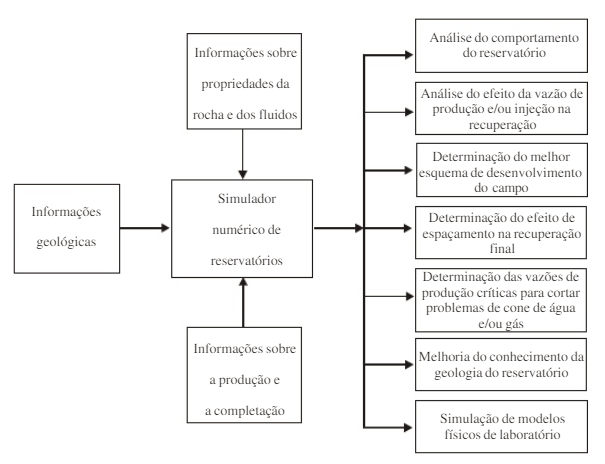
\includegraphics[width=.75\textwidth]{figs/revisao/revisao_simsec1}
	\caption{Aplica\c{c}\~{a}o de simuladores num\'{e}ricos em reservat\'{o}rios \cite[p. 522]{engres}}
	\label{fig:revisao_simsec1}
\end{figure}  

As etapas normalmente seguidas durante a simula\c{c}\~{a}o num\'{e}rica de um reservat\'{o}rio s\~{a}o \footnote{Ver \cite[pp. 523--524]{engres}. Ver tamb\'{e}m \cite{fanchi} para maiores detalhes sobre cada etapa.}:

\begin{enumerate}
\item \textbf{Coleta e prepara\c{c}\~{a}o dos dados:} \'{e} a fase de armazenamento e interpreta\c{c}\~{a}o de todos os dados cab\'{i}veis ao problema, sejam eles geol\'{o}gicos, propriedades da rocha e dos fluidos, entre outros. Quanto maiores a quantidade e a qualidade desses dados, mais confi\'{a}vel ser\'{a} a simula\c{c}\~{a}o. Breitenbach destaca que dados adicionais podem ser necess\'{a}rios considerando-se a dificuldade do problema de mec\^{a}nica dos fluidos e os objetivos de estudo, dependentes de qual processo do reservat\'{o}rio est\'{a} sendo modelado \cite{breitenbach1991}.
\item \textbf{Prepara\c{c}\~{a}o do modelo num\'{e}rico:} Ocorre logo ap\'{o}s a tomada dos dados. Inicialmente, \'{e} feito o \textit{lan\c{c}amento do} grid \textit{ou malha}, onde \'{e} constru\'{i}da uma malha para se transpor as informa\c{c}\~{o}es necess\'{a}rias para o modelo. Logo, \'{e} feita a divis\~{a}o do reservat\'{o}rio em v\'{a}rias c\'{e}lulas, cada uma funcionando como um reservat\'{o}rio menor, conforme mostra a Figura \ref{fig:revisao_simsec3}. Breitenbach ressalta que combina\c{c}\~{o}es de modelos muitas vezes s\~{a}o selecionadas para se estudar, por exemplo, posicionamento de po\c{c}os, fen\^{o}menos de cone, inje\c{c}\~{a}o de fluidos, vaz\~{o}es de produ\c{c}\~{a}o, etc., e que o engenheiro deve utilizar a dimens\~{a}o da malha e os modelos corretos para resolver o problema desejado com as restri\c{c}\~{o}es de custo, tempo e acur\'{a}cia consideradas \cite{breitenbach1991}.
\begin{figure}[H]
	\centering
	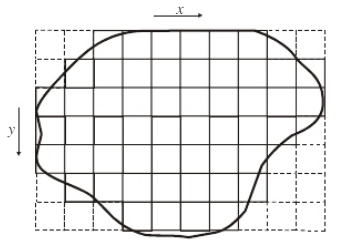
\includegraphics[width=.5\textwidth]{figs/revisao/revisao_simsec3}
	\caption{Malha utilizada na simula\c{c}\~{a}o num\'{e}rica de um reservat\'{o}rio \cite[p. 524]{engres}}
	\label{fig:revisao_simsec3}
\end{figure}
\item \textbf{Ajuste de hist\'{o}rico:} O objetivo desta etapa \'{e} calibrar o modelo num\'{e}rico com o reservat\'{o}rio real a partir dos melhores dados dispon\'{i}veis referentes aos hist\'{o}ricos de produ\c{c}\~{a}o e de press\~{a}o. Oliver e Chen afirmam que se trata de um problema inverso: ao inv\'{e}s de se obter um modelo de reservat\'{o}rio para predizer seu comportamento, a modelagem \'{e} feita a partir da observa\c{c}\~{a}o dos processos ocorridos no reservat\'{o}rio \cite{Oliver2011}\footnote{Oliver e Chen apresentam uma revis\~{a}o da literatura a respeito do ajuste de hist\'{o}rico; ver \cite{Oliver2011}}. O ajuste de hist\'{o}rico \'{e} um c\'{a}lculo do comportamento passado do reservat\'{o}rio e a consequente compara\c{c}\~{a}o com o hist\'{o}rico do campo ou do mesmo reservat\'{o}rio; se a concord\^{a}ncia n\~{a}o \'{e} satisfat\'{o}ria, s\~{a}o necess\'{a}rios ajustes nos dados at\'{e} se obter resultados adequados. De todo modo, a import\^{a}ncia de se obter um bom ajuste de hist\'{o}rico reside no fato de que o modelo poder\'{a} ser utilizado para se efetuar previs\~{o}es confi\'{a}veis em rela\c{c}\~{a}o ao seu comportamento futuro.
\item \textbf{Extrapola\c{c}\~{a}o:} Uma vez que o ajuste de hist\'{o}rico \'{e} realizado, procede-se \`{a} fase de extrapola\c{c}\~{a}o, isto \'{e}, a previs\~{a}o de comportamento futuro do modelo. Podem ser impostas vaz\~{o}es e press\~{o}es para todos os po\c{c}os, condi\c{c}\~{o}es dessas vaz\~{o}es, entre outros. Essa etapa permite avaliar v\'{a}rios esquemas de produ\c{c}\~{a}o, e seus resultados podem ser utilizados em avalia\c{c}\~{o}es econ\^{o}micas, tornando poss\'{i}vel decidir pelo esquema \'{o}timo de produ\c{c}\~{a}o, conforme tamb\'{e}m sugere Fanchi \footnote{Ver \cite[p. 373]{fanchi}.}.
\end{enumerate}

Todas as etapas de simula\c{c}\~{a}o num\'{e}rica de reservat\'{o}rios est\~{a}o resumidos na Figura \ref{fig:revisao_simsec2}.

\begin{figure}[!ht]
	\centering
	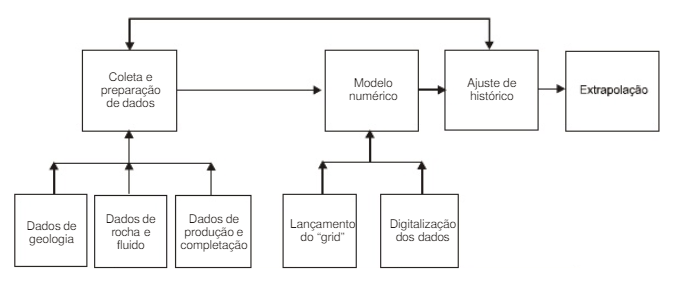
\includegraphics[width=.75\textwidth]{figs/revisao/revisao_simsec2}
	\caption{Etapas da simula\c{c}\~{a}o num\'{e}rica de um reservat\'{o}rio \cite[p. 523]{engres}}
	\label{fig:revisao_simsec2}
\end{figure}